\section{Resultados y Análisis}

\subsection{Continuos}

\begin{frame}
    \frametitle{Ranking en continuos para fitness}
    \begin{columns}
        \column{0.5\textwidth}
        \begin{figure}
            \begin{center}
                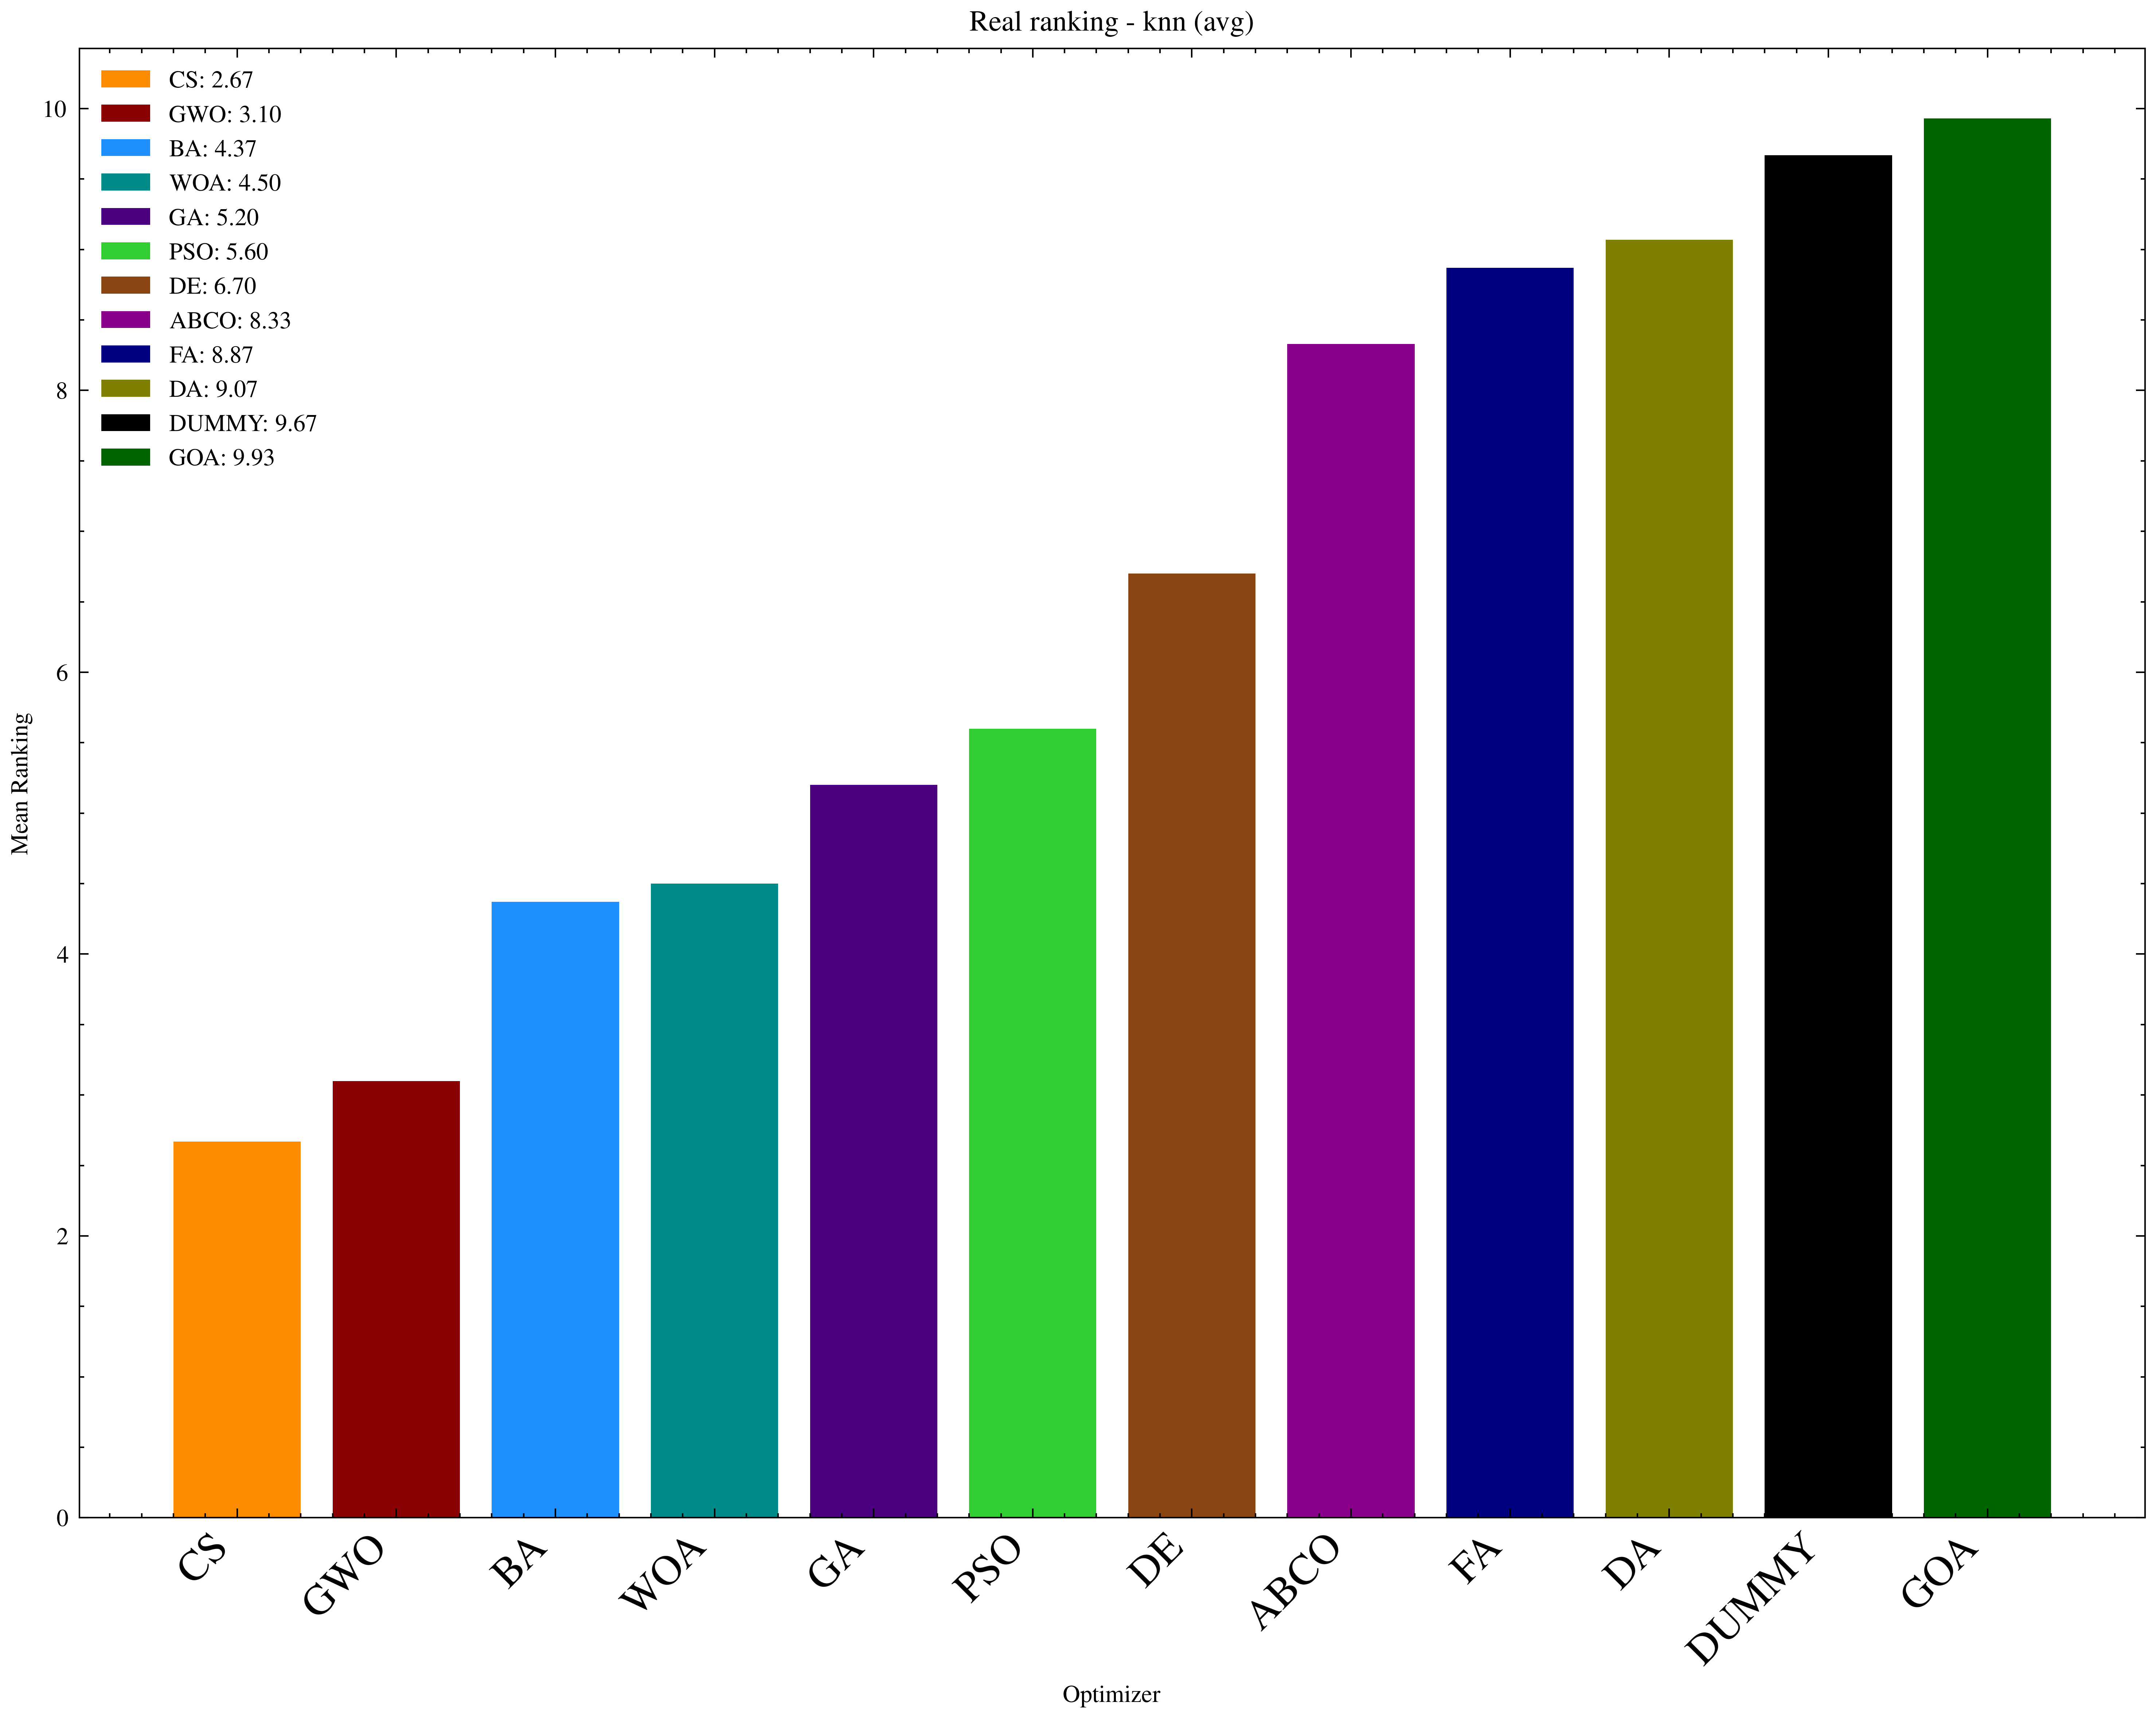
\includegraphics[width=0.8\textwidth]{imagenes/chapter5/rankings_knn_avg_real.png}
            \end{center}
            \caption{Ranking de los algoritmos en versión continua para kNN}
        \end{figure}
        \column{0.5\textwidth}
        \begin{figure}
            \begin{center}
                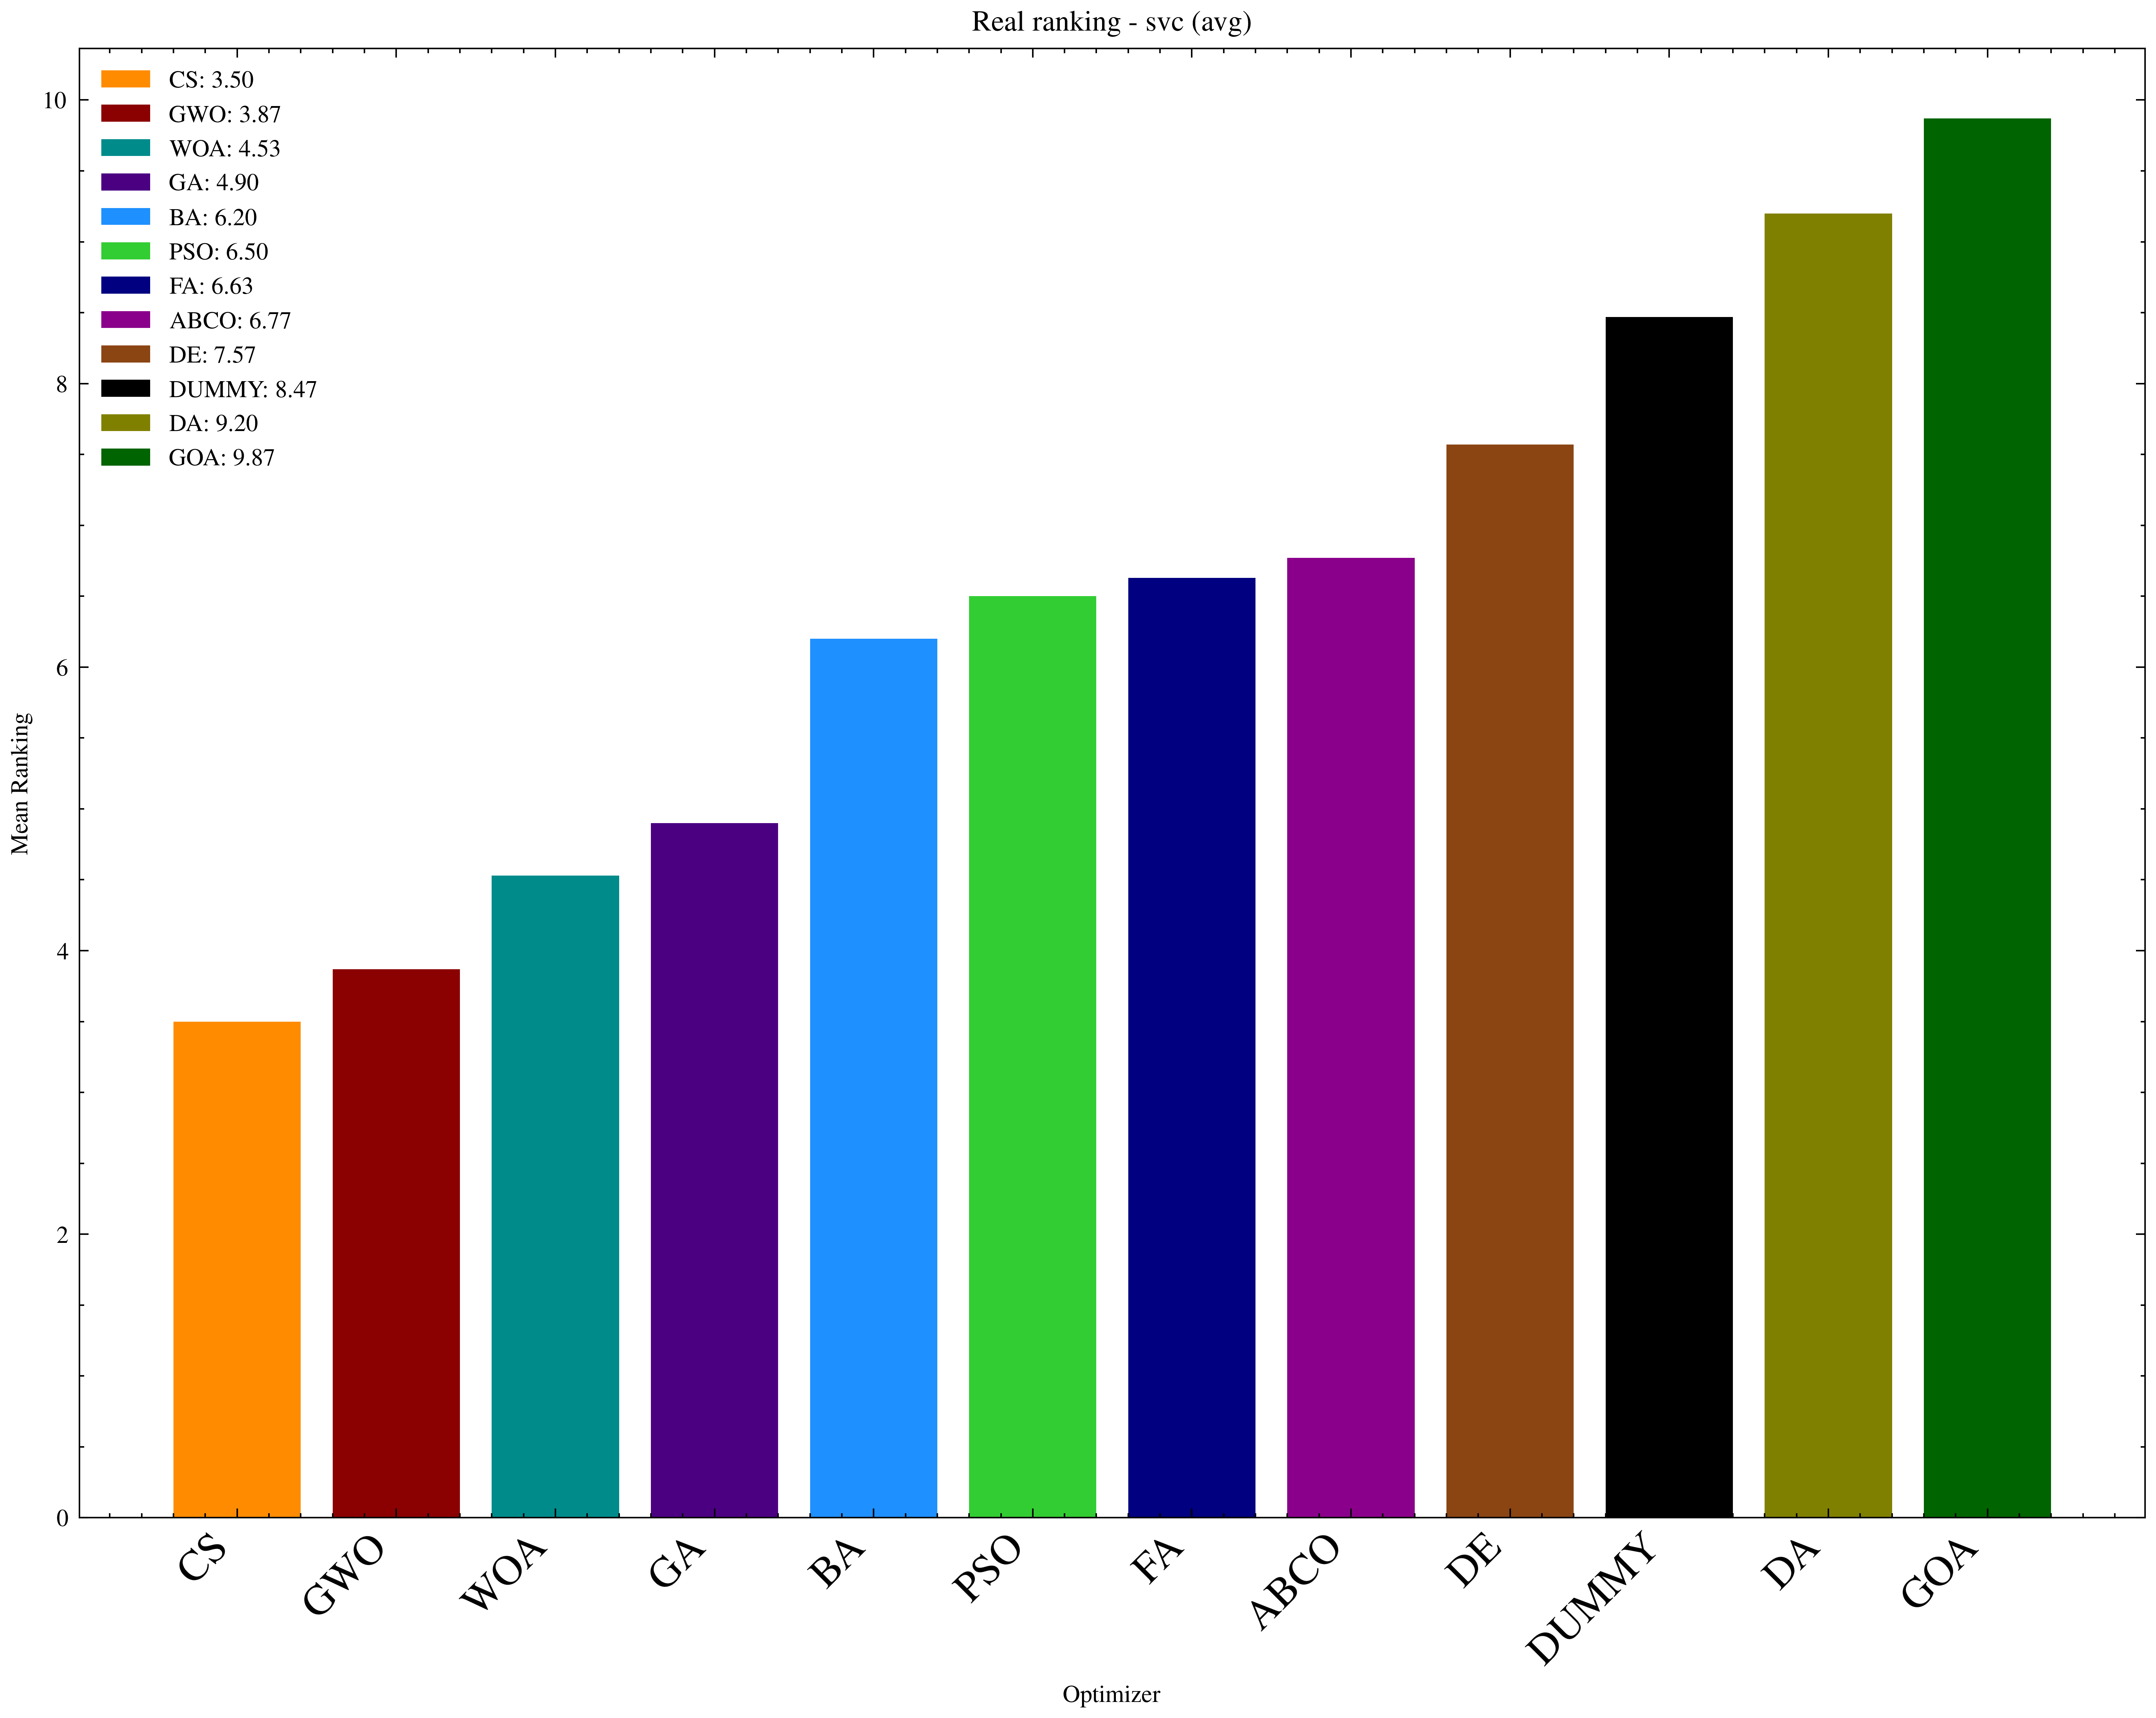
\includegraphics[width=0.8\textwidth]{imagenes/chapter5/rankings_svc_avg_real.png}
            \end{center}
            \caption{Ranking de los algoritmos en versión continua para SVC}
        \end{figure}
    \end{columns}
\end{frame}

\begin{frame}
    \frametitle{Resultados en continuos}
    \begin{enumerate}
        \item Los mejores algoritmos en \textit{fitness} son \textbf{CS} y \textbf{GWO}. Los peores algoritmos son \textbf{GOA} y \textbf{DA}.
        \item Los mejores reduciendo características vuelven a ser \textbf{CS} y \textbf{GWO}. Además con mucha diferencia.
        \item El algoritmo más rápido es \textbf{FA}, mientras que el más lento es \textbf{ABCO}.
    \end{enumerate}
\end{frame}


\begin{frame}
    \frametitle{Convergencia en continuo}
    \begin{columns}
        \column{0.5\textwidth}
        \begin{figure}[htp]
            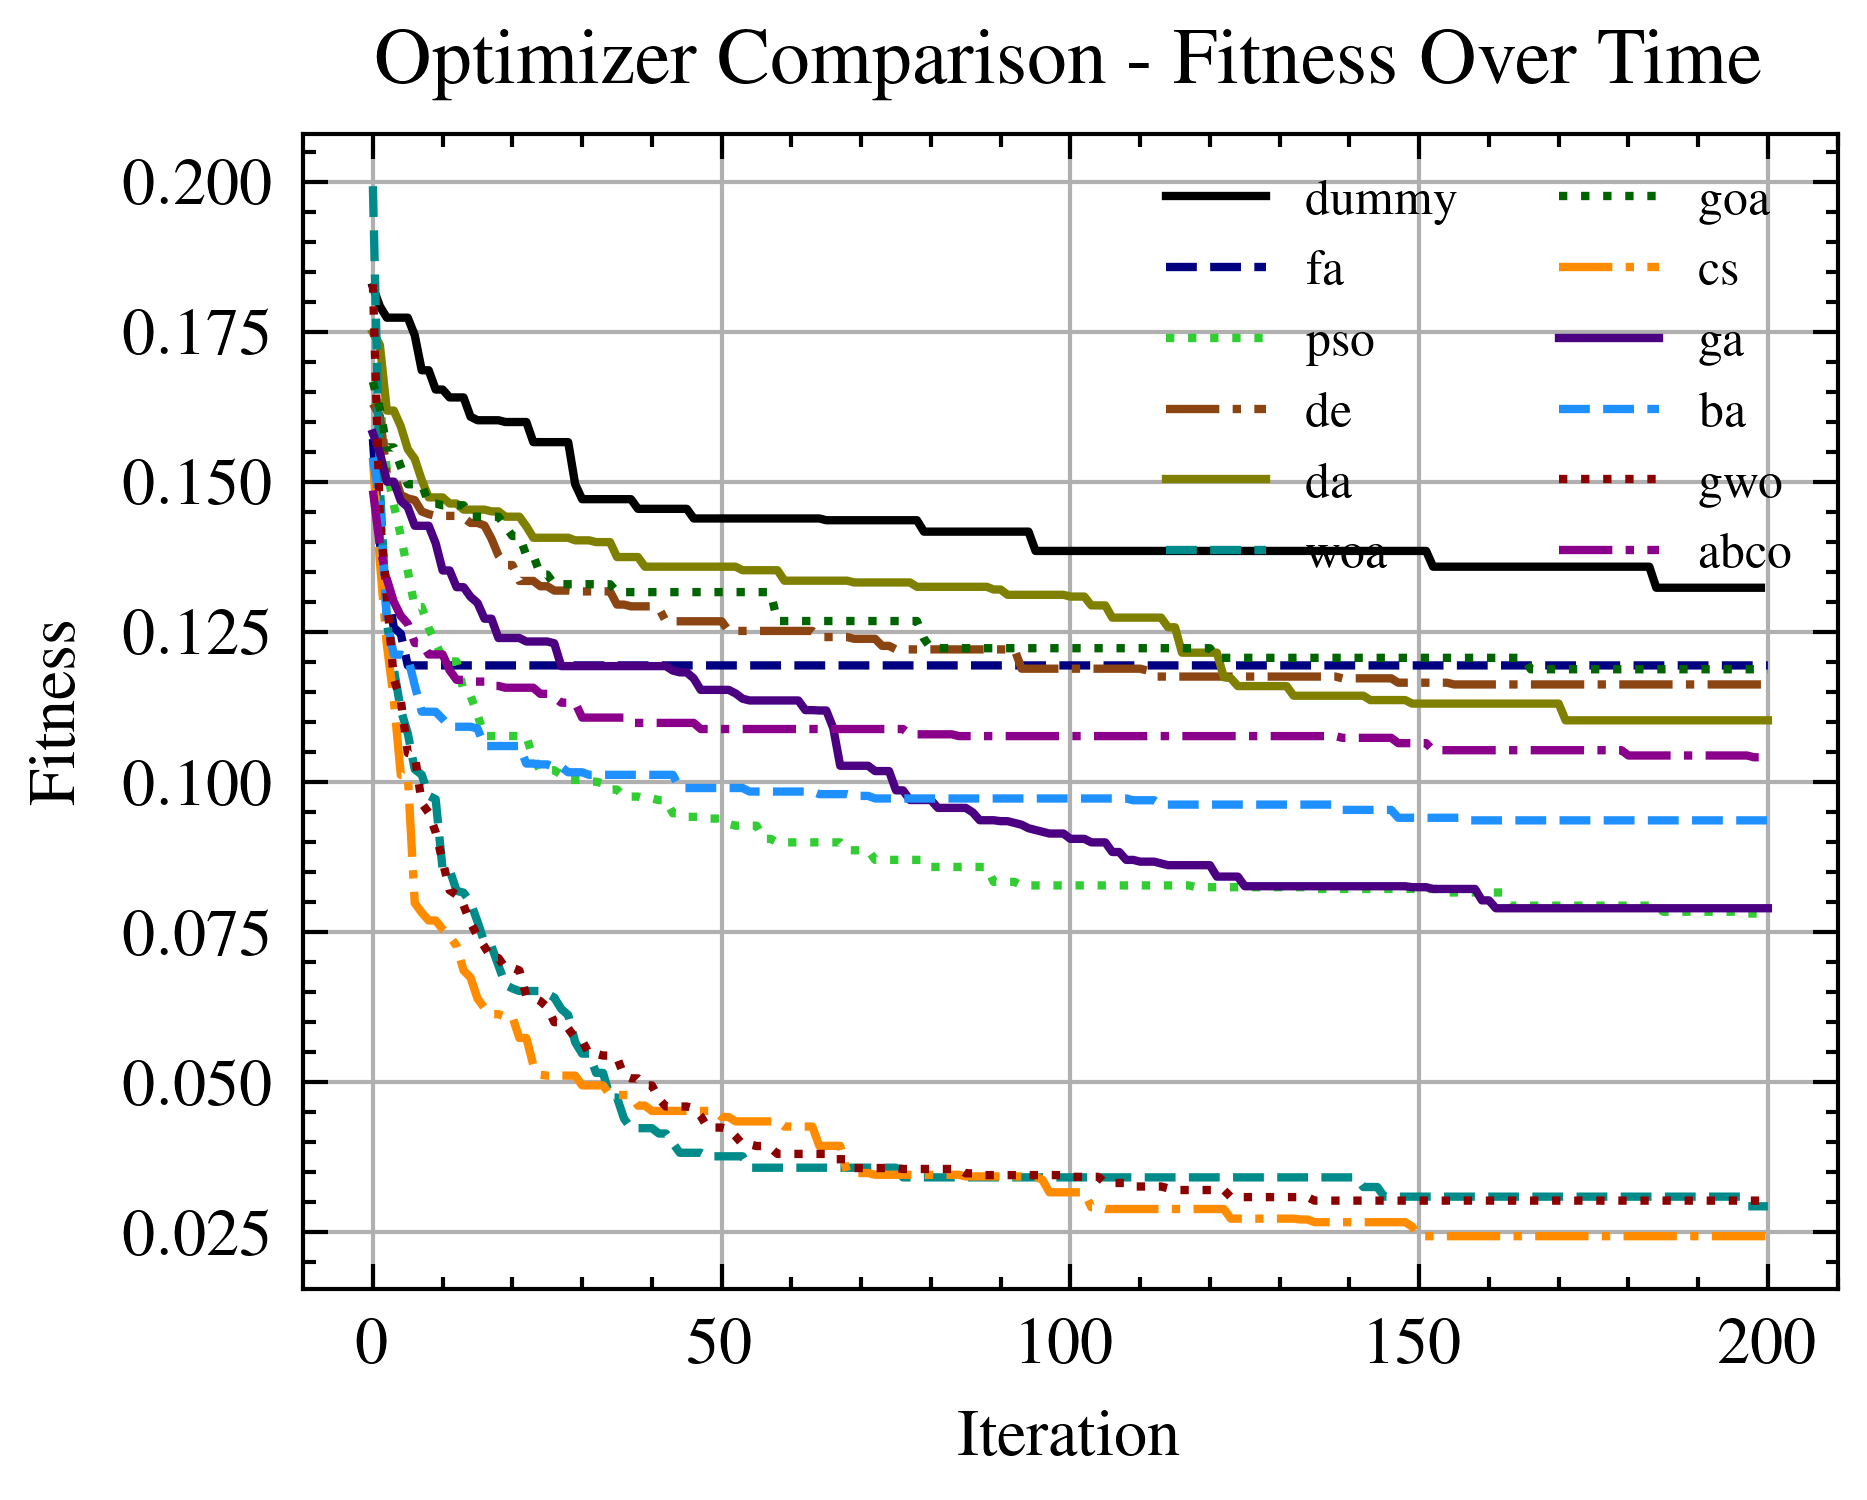
\includegraphics[width=0.8\textwidth]{imagenes/chapter5/optimizers_fitness_knn_io.png}
            \caption{Convergencia de todas las metaheurísticas en ionosphere - knn - real}
        \end{figure}
        \column{0.5\textwidth}
        \begin{figure}[htp]
            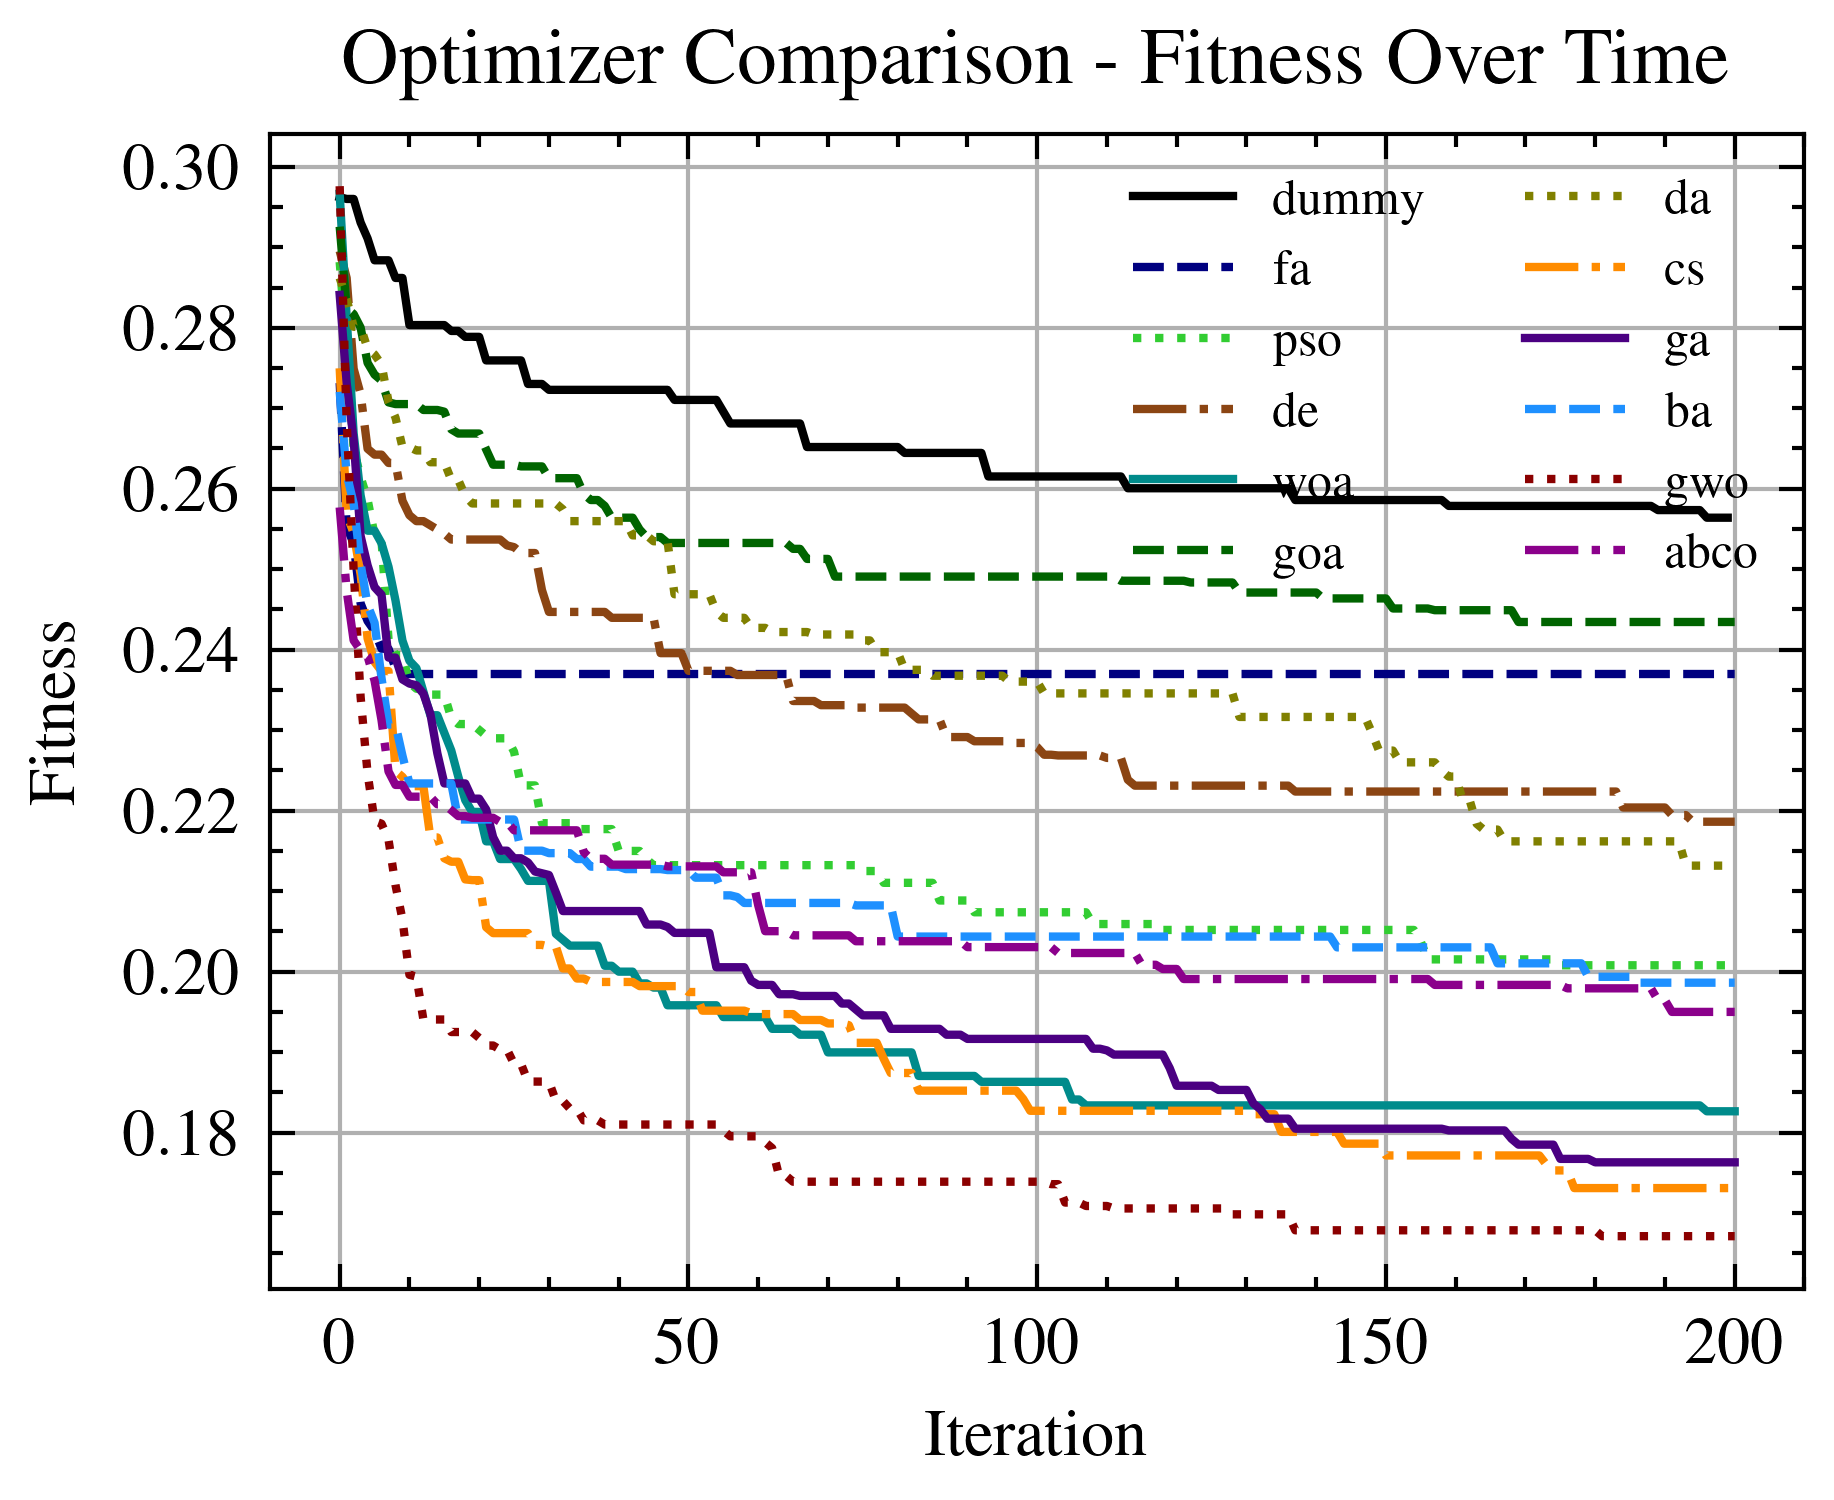
\includegraphics[width=0.8\textwidth]{imagenes/chapter5/optimizers_fitness_knn_dia.png}
            \caption{Convergencia de todas las metaheurísticas en diabetes - knn - real}
        \end{figure}
    \end{columns}
\end{frame}


\subsection{Binarios}
\begin{frame}
    \frametitle{Ranking en binario para fitness}
    \begin{columns}
        \column{0.5\textwidth}
        \begin{figure}
            \begin{center}
                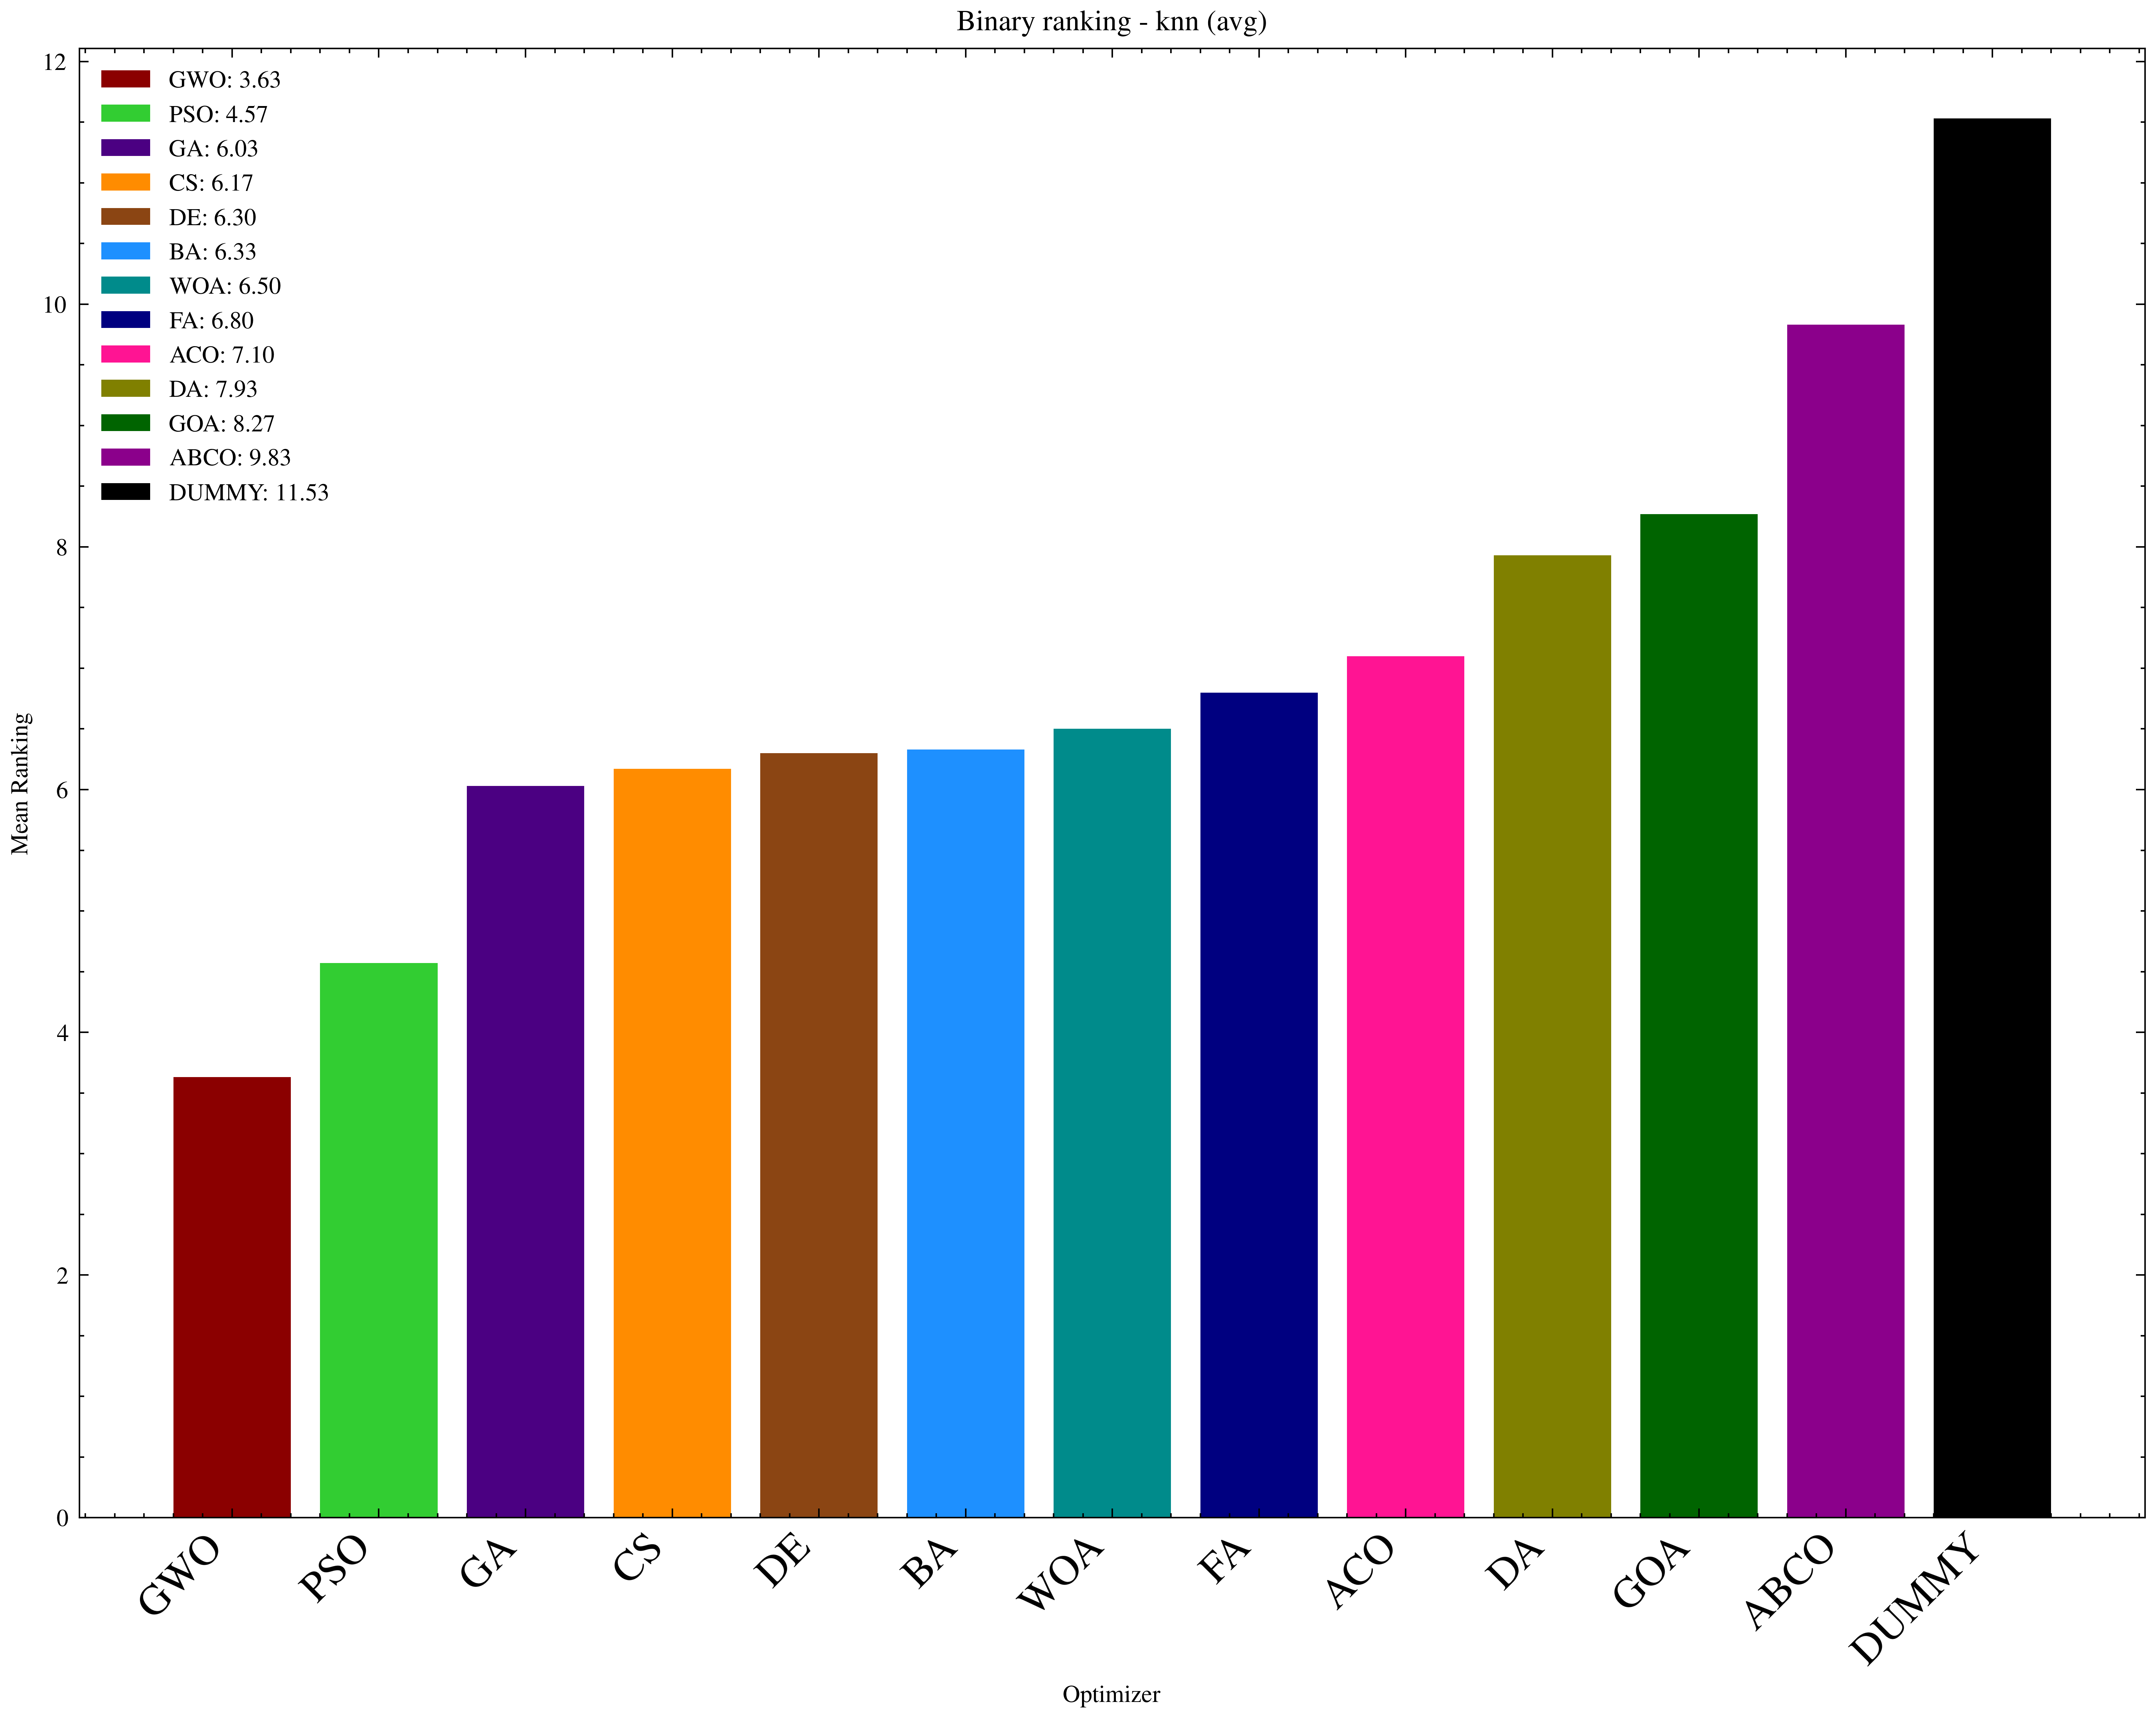
\includegraphics[width=0.8\textwidth]{imagenes/chapter5/rankings_knn_avg_bin.png}
            \end{center}
            \caption{Ranking de los algoritmos en versión binaria para kNN}
        \end{figure}
        \column{0.5\textwidth}
        \begin{figure}
            \begin{center}
                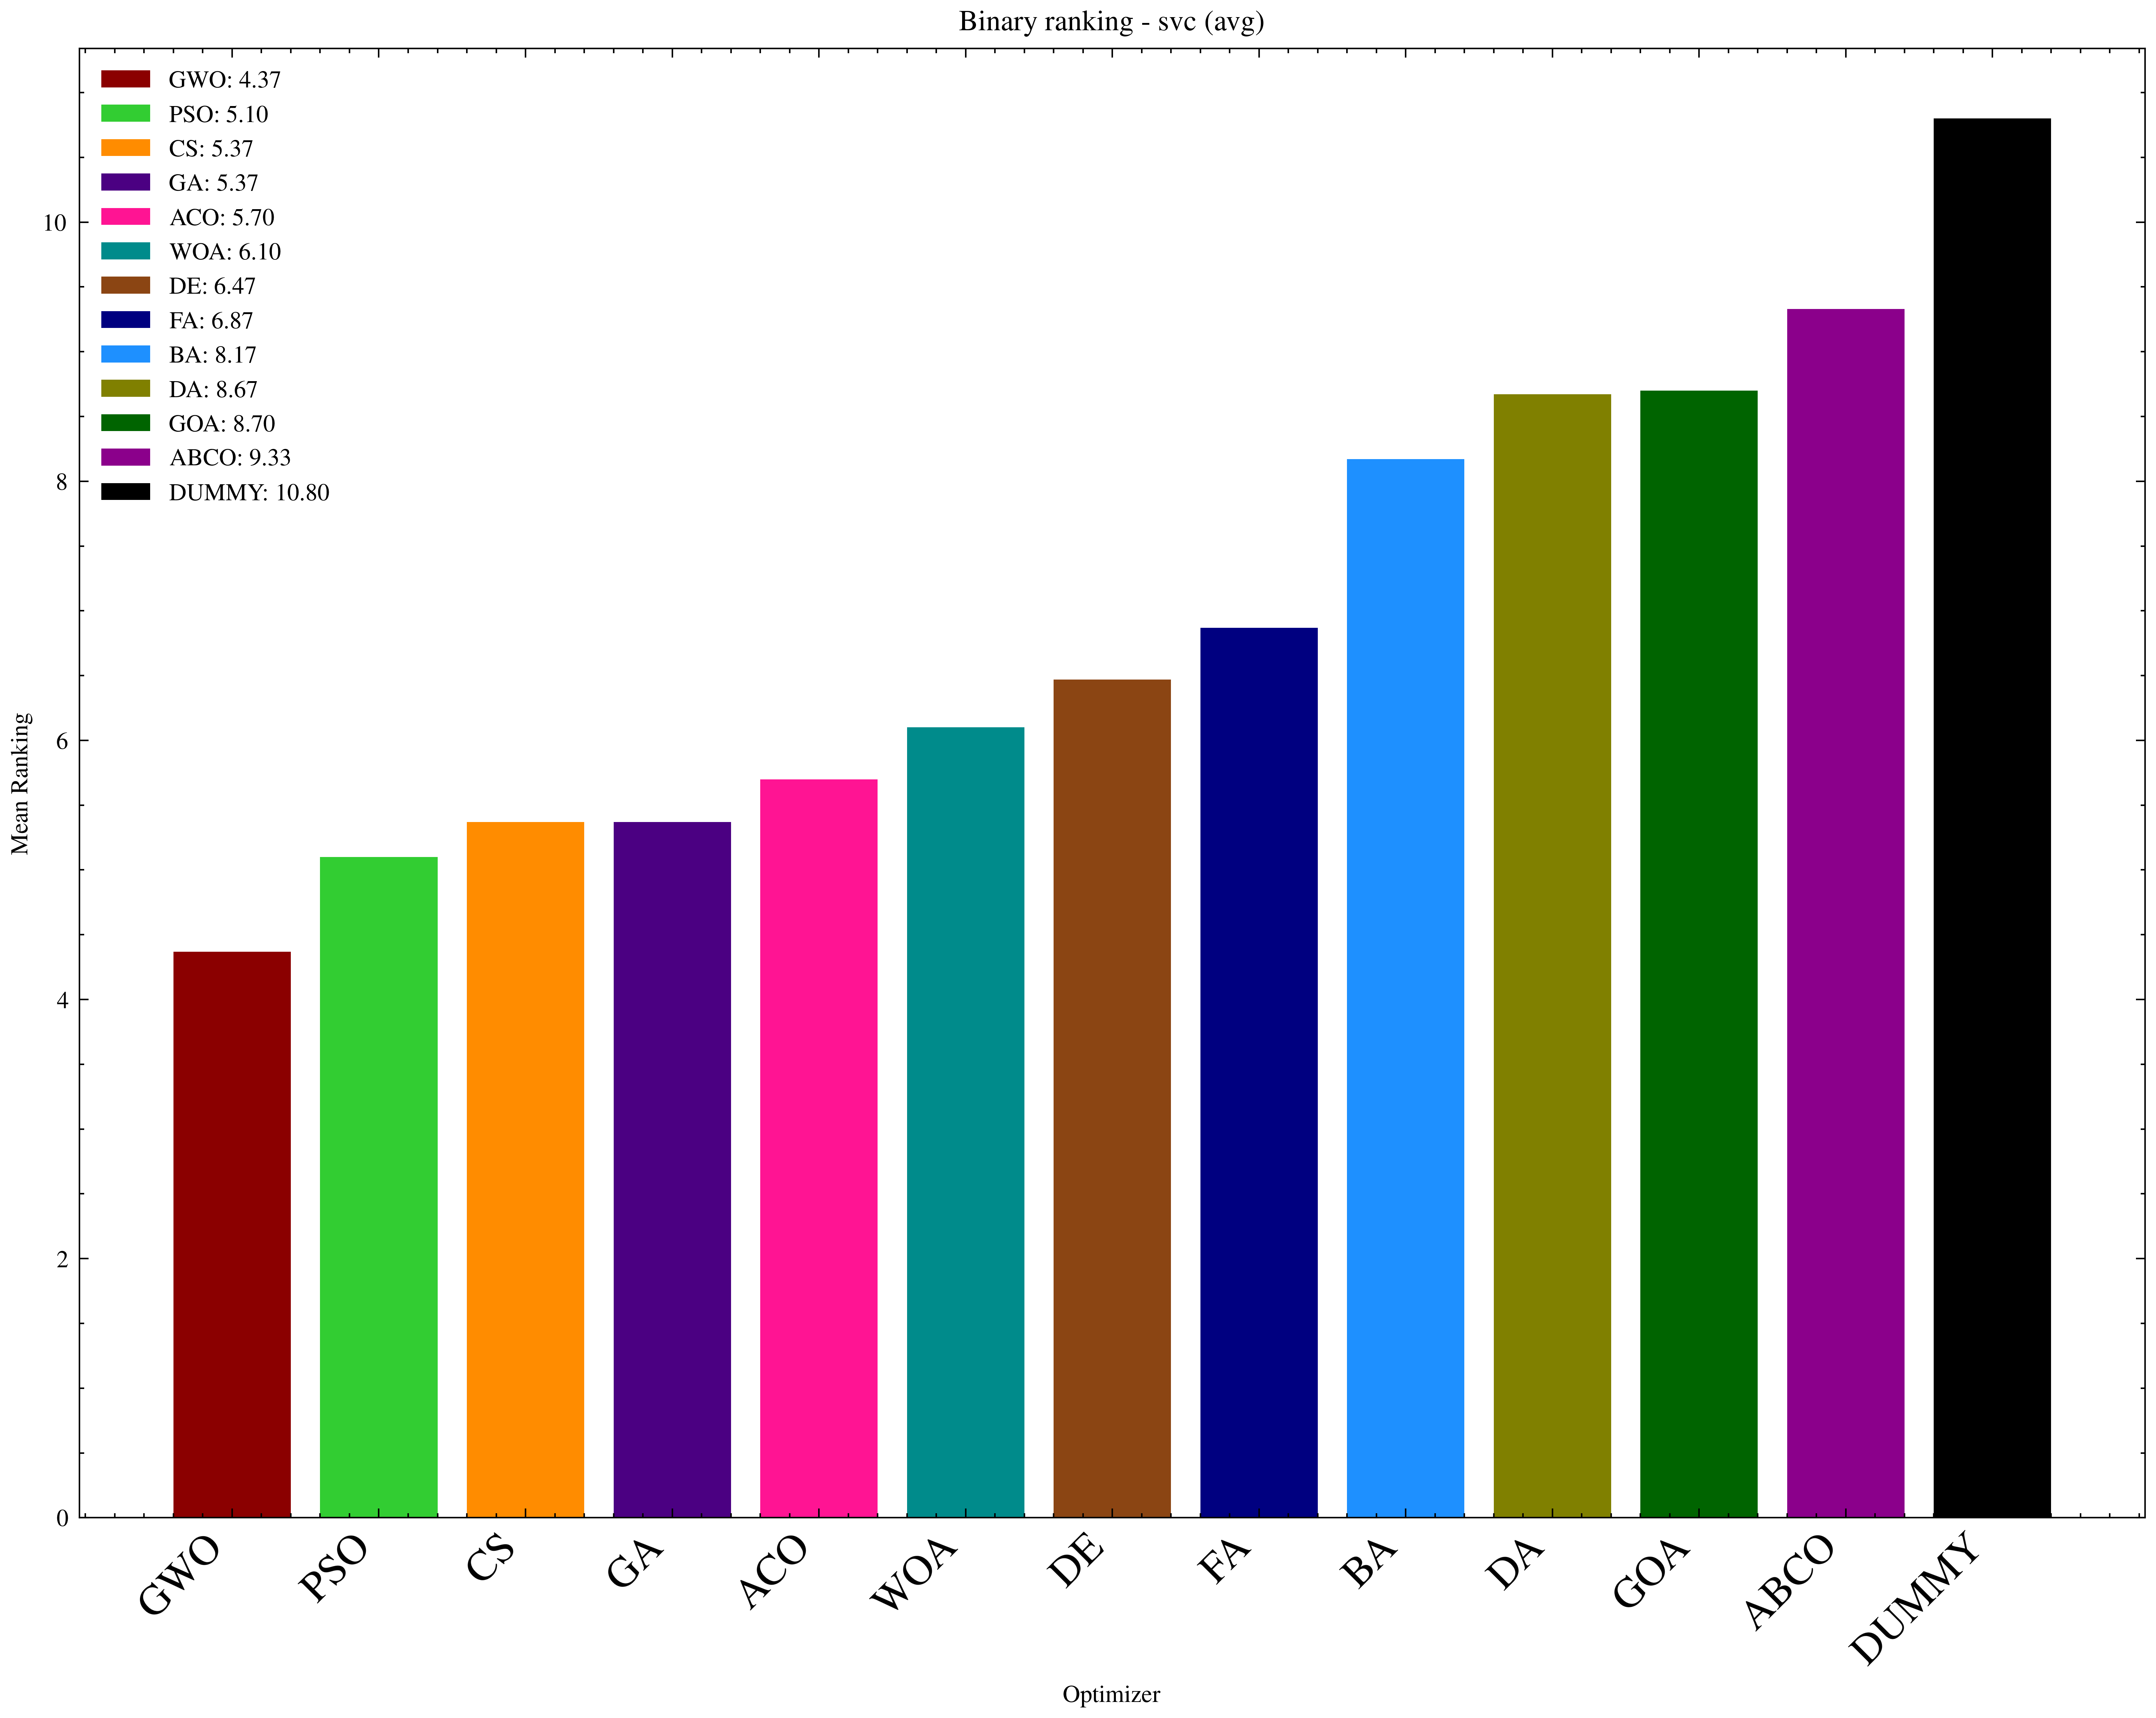
\includegraphics[width=0.8\textwidth]{imagenes/chapter5/rankings_svc_avg_bin.png}
            \end{center}
            \caption{Ranking de los algoritmos en versión binaria para SVC}
        \end{figure}
    \end{columns}
\end{frame}

\begin{frame}
    \frametitle{Resultados en binarios}
    \begin{enumerate}
        \item Los mejores algoritmos en \textit{fitness} son \textbf{bGWO} y \textbf{bPSO}. Los peores algoritmos son \textbf{bGOA} y \textbf{bABCO}.
        \item El mejor reduciendo características es \textbf{ACO}.
        \item El algoritmo más rápido vuelve a ser \textbf{bFA}. Ocurre igual con el más lento, que es \textbf{ABCO}.
    \end{enumerate}
\end{frame}